%%%%%%%%%%%%%%%%%%%%%%%%%%%%%%%%%%%%%%%%%%%%%%%%%%%%%%%%%%
% # Examination of Variance in the SPRT and AJT Response Data
%%%%%%%%%%%%%%%%%%%%%%%%%%%%%%%%%%%%%%%%%%%%%%%%%%%%%%%%%%

\chapter{Examination of Variance in the SPRT and AJT Response Data}\label{ch-variance}

This chapter examines variance in participants' SPRT comprehension-question accuracy data and AJT rating data in order to determine whether they had trouble judging the acceptability of sentences that could not be straightforwardly traced to parsing difficulty. The presence of non-parsing-related difficulty in assigning ratings to sentences would support the entrenchment approach the formation of well-formedness perceptions described in Section~\ref{acq-entrenchment}, especially if the severity of that difficulty shrinks with rising L2 proficiency scores. Section~\ref{var-rq} lays out the research questions (RQs) for the chapter, Sections~\ref{var-spr}--\ref{var-ajt-proficiency} walk the reader through the results from each of the data analyses, and Section~\ref{var-conclusion} concludes the chapter.

%========================================================%
\section{Research questions}\label{var-rq}
%========================================================%

My RQs for this chapter were as follows:

\begin{enumerate}[\bfseries RQ1:,itemsep=5pt]
\item {\bfseries How does variance in SPRT responses pattern across the SLW hierarchy?}\par\nobreak
Prediction: Variance will be smaller in RP trials than in gap trials, at least at lower levels on the hierarchy. I would take such a pattern of results as yet another source of evidence that resumption facilitates parsing of RCs under processing strain.
\end{enumerate}\vspace{5pt}

\begin{enumerate}[\bfseries RQ2:,itemsep=5pt]
\item {\bfseries How does variance in AJT responses pattern across the SLW hierarchy?}\par\nobreak
Prediction: Variance in RP trials will be at least as large as variance in gap trials for all levels on the hierarchy. Such a pattern of results would suggest that participants experienced difficulty assigning ratings to RP trials above and beyond what can be explained in terms of parsing problems.
\end{enumerate}\vspace{5pt}

\begin{enumerate}[\bfseries RQ3:,itemsep=5pt]
\item {\bfseries How does L2 proficiency affect variance in participants' responses?}\par\nobreak
Prediction: The variance observed in participants' responses will shrink as proficiency scores get higher. In the SPRT response data, this would indicate that processing in general is more efficient for L2ers with higher levels of English ability than for those with lower levels of English ability. In the AJT response data, it would additionally suggest that perceptions of well-formedness come into sharper focus as proficiency increases.
\end{enumerate}

%========================================================%
\section{SPRT variance data}\label{var-spr}
%========================================================%

To address RQ1, I examined how variance in participants' SPRT comprehension-question accuracy scores patterned across the SLW hierarchy. I calculated variances by participant such that each individual had one variance score for each critical condition. Figures \ref{fig:orc-spr-var} and \ref{fig:src-spr-var} show the mean variance in comprehension-question accuracy for the ORC and SRC datasets, respectively. 

\begin{figure}
\caption{Mean variance for comprehension-question accuracy in the ORC self-paced reading task} \label{fig:orc-spr-var}
\raggedright\setstretch{1}
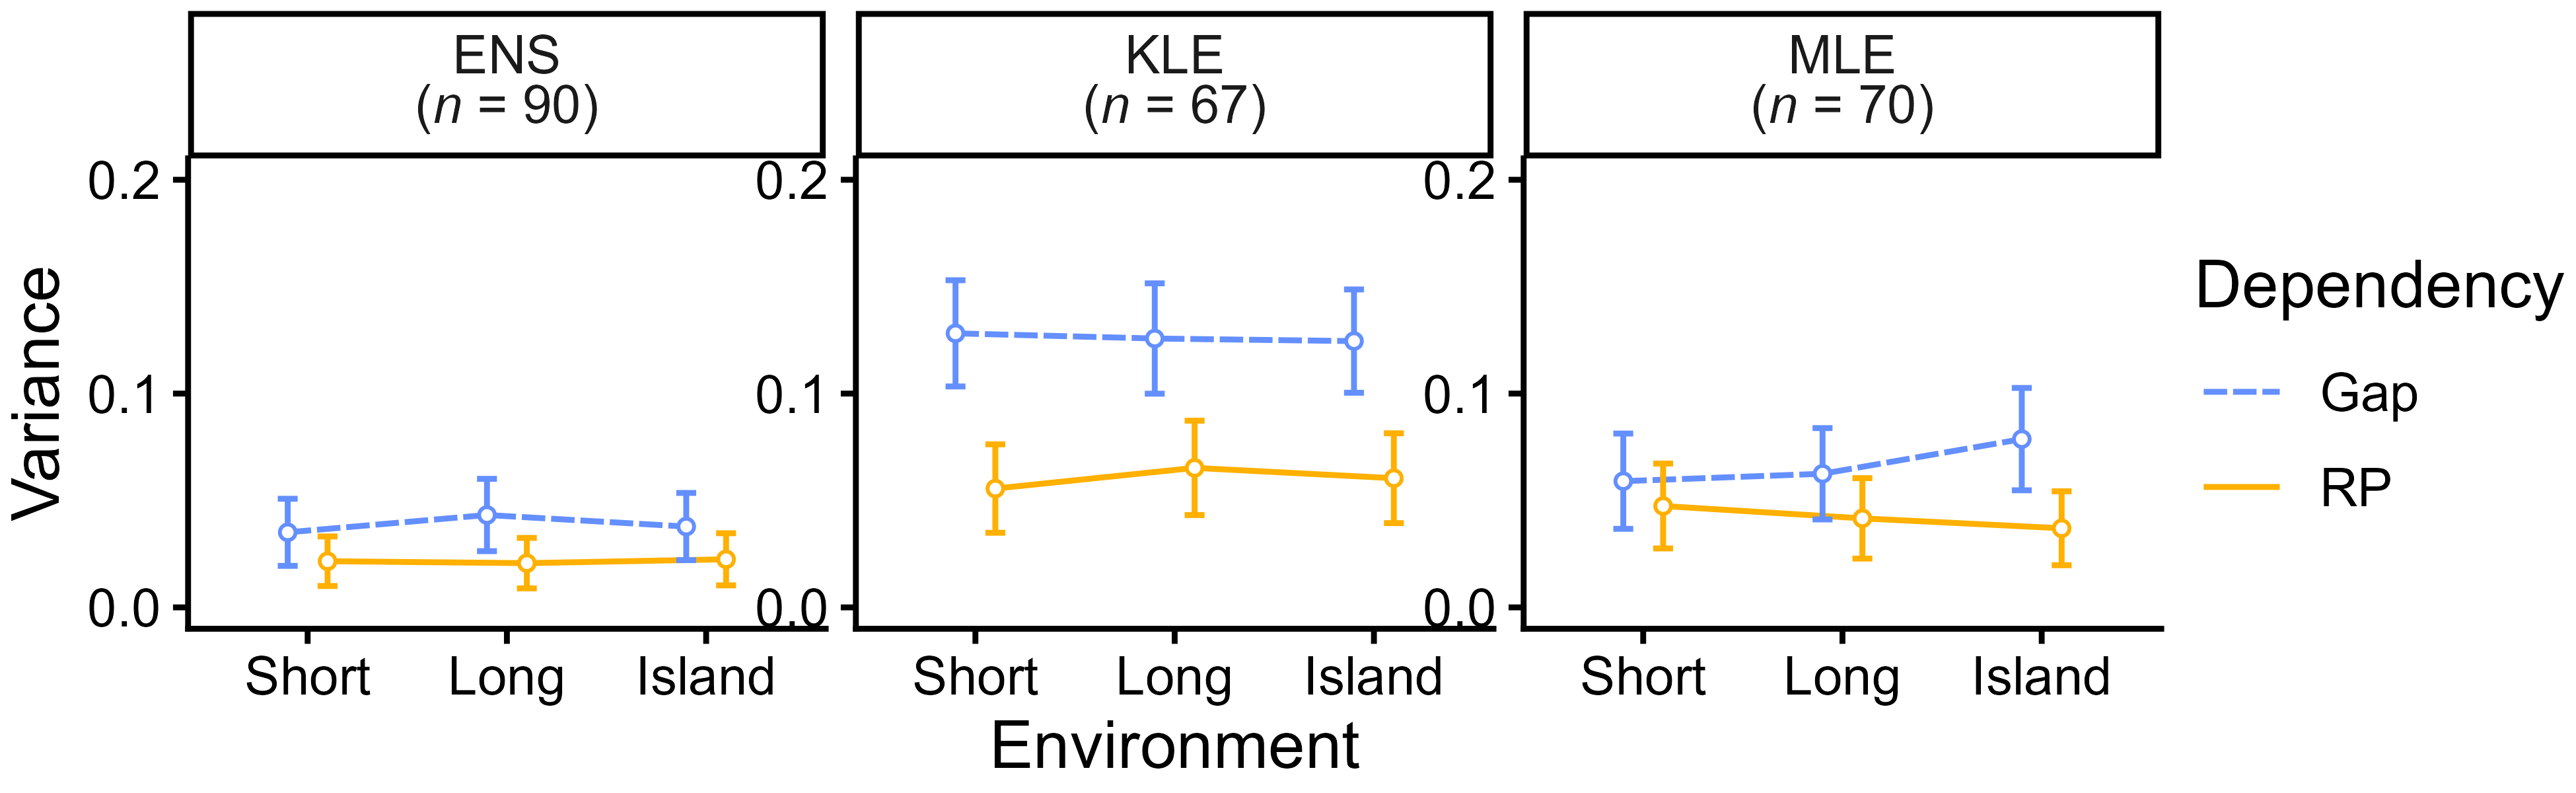
\includegraphics{../analysis/plots/orc_spr_accuracy_var.png}
\vspace{-12pt}
\end{figure}

\begin{figure}
\caption{Mean variance for comprehension-question accuracy in the SRC self-paced reading task} \label{fig:src-spr-var}
\raggedright\setstretch{1}
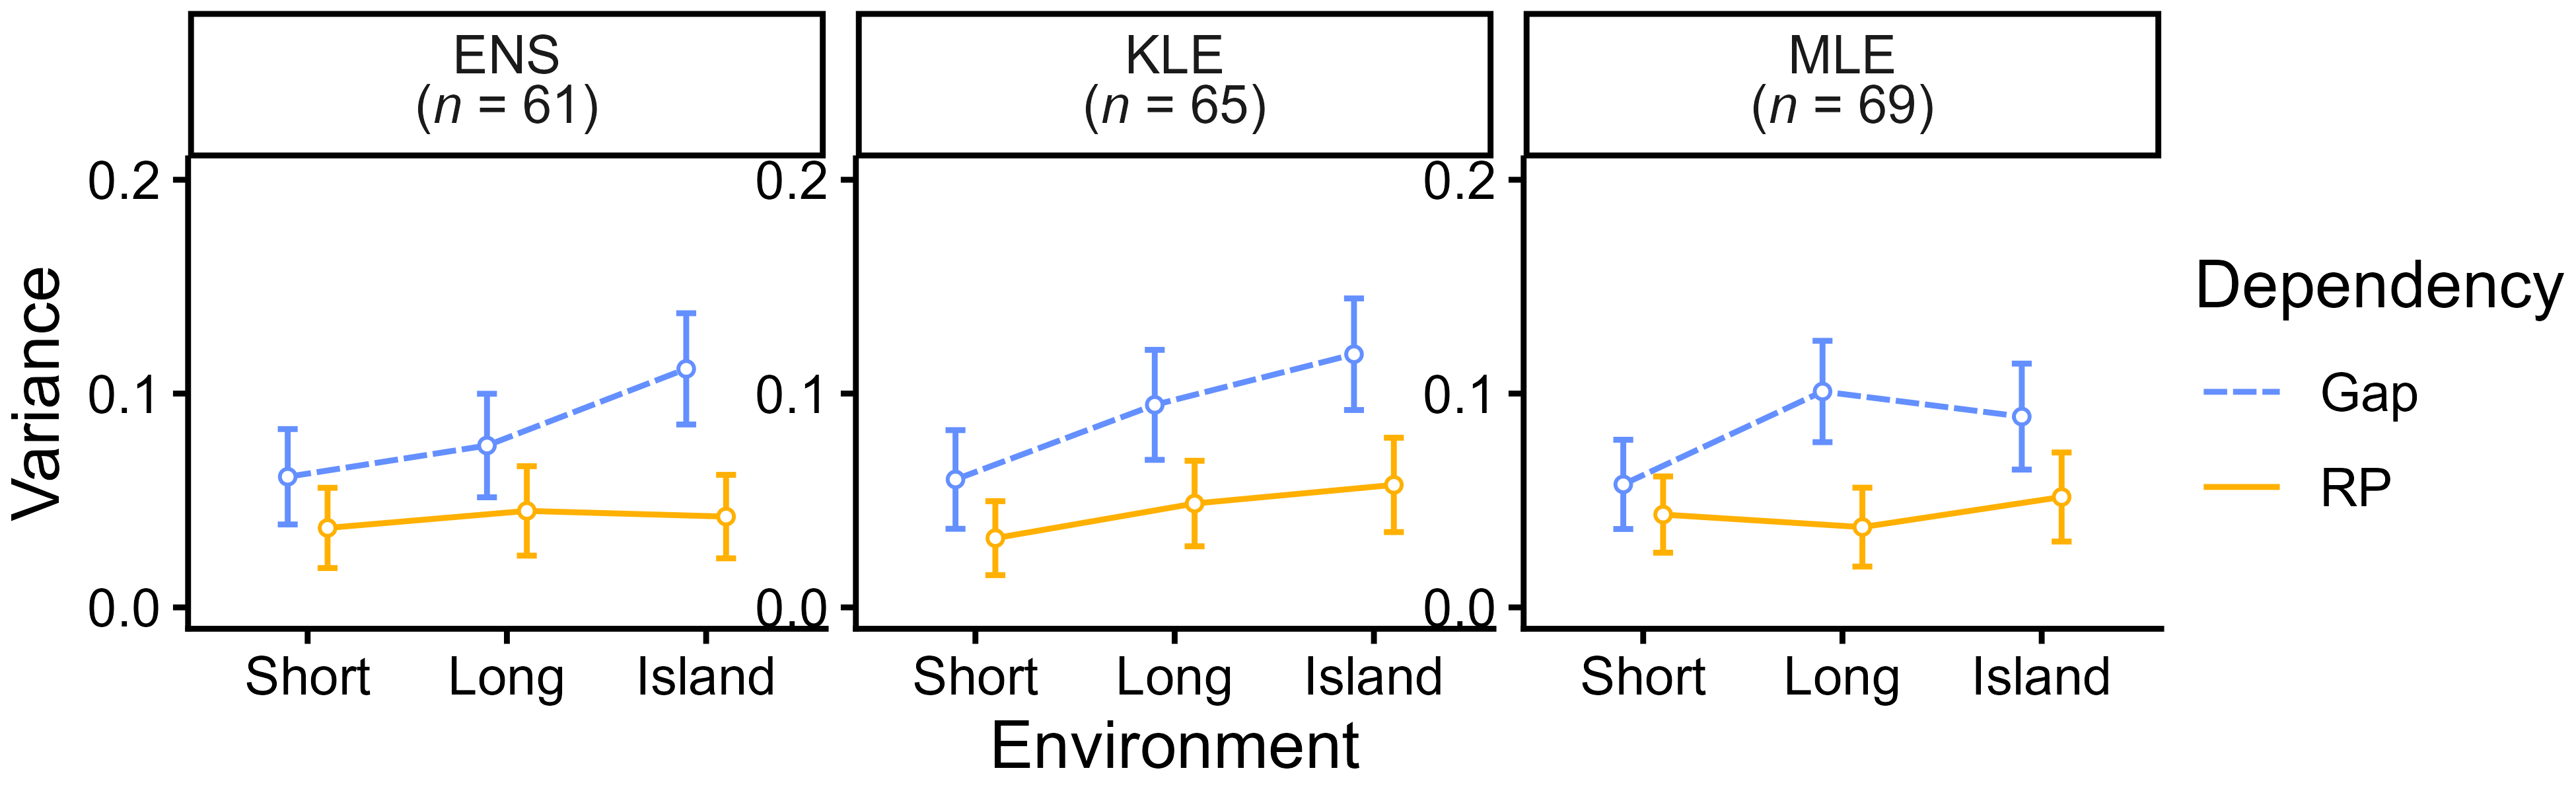
\includegraphics{../analysis/plots/src_spr_accuracy_var.png}
\vspace{-12pt}
\end{figure}

\noindent The mean variance was smaller for RPs than for gaps across all combinations of \textsc{environment} and \textsc{group}, and the [RP~−~gap] contrast tended to be greater in the Long and Island conditions, where processing should be harder, than in the Short condition, where processing should be easier. The pattern displayed in the variance data is, in short, the direct inverse of the pattern displayed in the accuracy data presented in Section~\ref{spr-accuracy}. That is to say that variance was lowest where accuracy was highest and vice versa.

I examined the variance scores in more detail by fitting them to separate linear mixed-effects models for the ORC and SRC datasets. The ORC model (model formula: \textsc{variance \~{} dependency * environment * group + (1 + dependency + environment | participant)}---see Table \ref{tblr:app-orc-spr-var-model} in the appendices for details) turned up significant effects for \textsc{dependency}, with variances being smaller for RPs than for gaps ($\hat{\beta}$~=~−0.04, \textit{SE}~=~0.00, $p$~<~.001), and for \textsc{group}, with KLEs and MLEs both having larger variances than ENSs (KLE~−~ENS: $\hat{\beta}$~=~0.06, \textit{SE}~=~0.01, $p$~<~.001; MLE~−~ENS: $\hat{\beta}$~=~0.02, \textit{SE}~=~0.01, $p$~=~.003). The \textsc{dependency}[RP] × \textsc{group}[KLE] interaction was also significant, indicating that the RP advantage was larger in scale for KLEs than it was for ENSs. Pairwise comparisons showed that the [RP~−~gap] contrast rose to significance for KLEs in all three environments (all $p$s~<~.001) and for MLEs only in the Island condition ($\hat{\beta}$~=~−0.04, \textit{SE}~=~0.01, $p$~=~.004). The contrast did not approach significance for ENSs in any of the environments tested, though; this was likely because variances were close to floor across all conditions in the ENS data.

The SRC model (model formula: \textsc{variance \~{} dependency * environment * group + (1 + dependency + environment | participant)}---see Table \ref{tblr:app-src-spr-var-model} in the appendices for details) found significant effects for \textsc{dependency}, with variances being smaller for RPs than for gaps ($\hat{\beta}$~=~−0.04, \textit{SE}~=~0.00, $p$~<~.001), and for \textsc{environment}, with variances being larger in both the Long and Island conditions than they were in the Short condition (Long~−~Short: $\hat{\beta}$~=~0.02, \textit{SE}~=~0.01, $p$~<~.001; Island~−~Short: $\hat{\beta}$~=~0.03, \textit{SE}~=~0.01, $p$~<~.001). The \textsc{dependency} × \textsc{environment} interactions were also significant, indicating that the RP advantage in variances was larger in the Long and Island conditions than it was in the Short condition (both $p$s~<~.05). Pairwise comparisons showed that the [RP~−~gap] contrast rose to significance for all groups in the Island condition (ENS: $\hat{\beta}$~=~−0.07, \textit{SE}~=~0.01, $p$~<~.001; KLE: $\hat{\beta}$~=~−0.06, \textit{SE}~=~0.01, $p$~<~.001; MLE: $\hat{\beta}$~=~−0.04, \textit{SE}~=~0.01, $p$~=~.037) and for L2ers also in the Long condition (KLE: $\hat{\beta}$~=~−0.05, \textit{SE}~=~0.01, $p$~=~.006; MLE: $\hat{\beta}$~=~−0.06, \textit{SE}~=~0.01, $p$~<~.001). For none of the groups did the contrast approach significance in the Short condition.

Overall, my analysis of the SPRT response data showed that variance was smaller for RPs than for gaps. This RP-over-gap advantage tended to be stronger towards the bottom of the SLW hierarchy, where processing should be harder, than at the top of the hierarchy, where processing should be easier. I take these results as evidence of yet another kind that resumption eases RC comprehension under processing strain. The fact that the variance data so closely mirrored the accuracy data presented in Section~\ref{spr-accuracy} indicates that variance can be used as a convenient proxy for difficulty---in this case, parsing difficulty.

%========================================================%
\section{L2 proficiency effects for the SPRT variance data}\label{var-spr-proficiency}
%========================================================%

Now let us examine the effect that L2 English proficiency had on the SPRT variance data. Figures~\ref{fig:orc-spr-var-proficiency} and \ref{fig:src-spr-var-proficiency} show the relationship between L2ers' SPRT variance scores and their scaled English proficiency scores in the ORC and SRC datasets, respectively.

\begin{figure}
\caption{L2 proficiency effects on variance scores in the ORC self-paced reading task} \label{fig:orc-spr-var-proficiency}
\raggedright\setstretch{1}
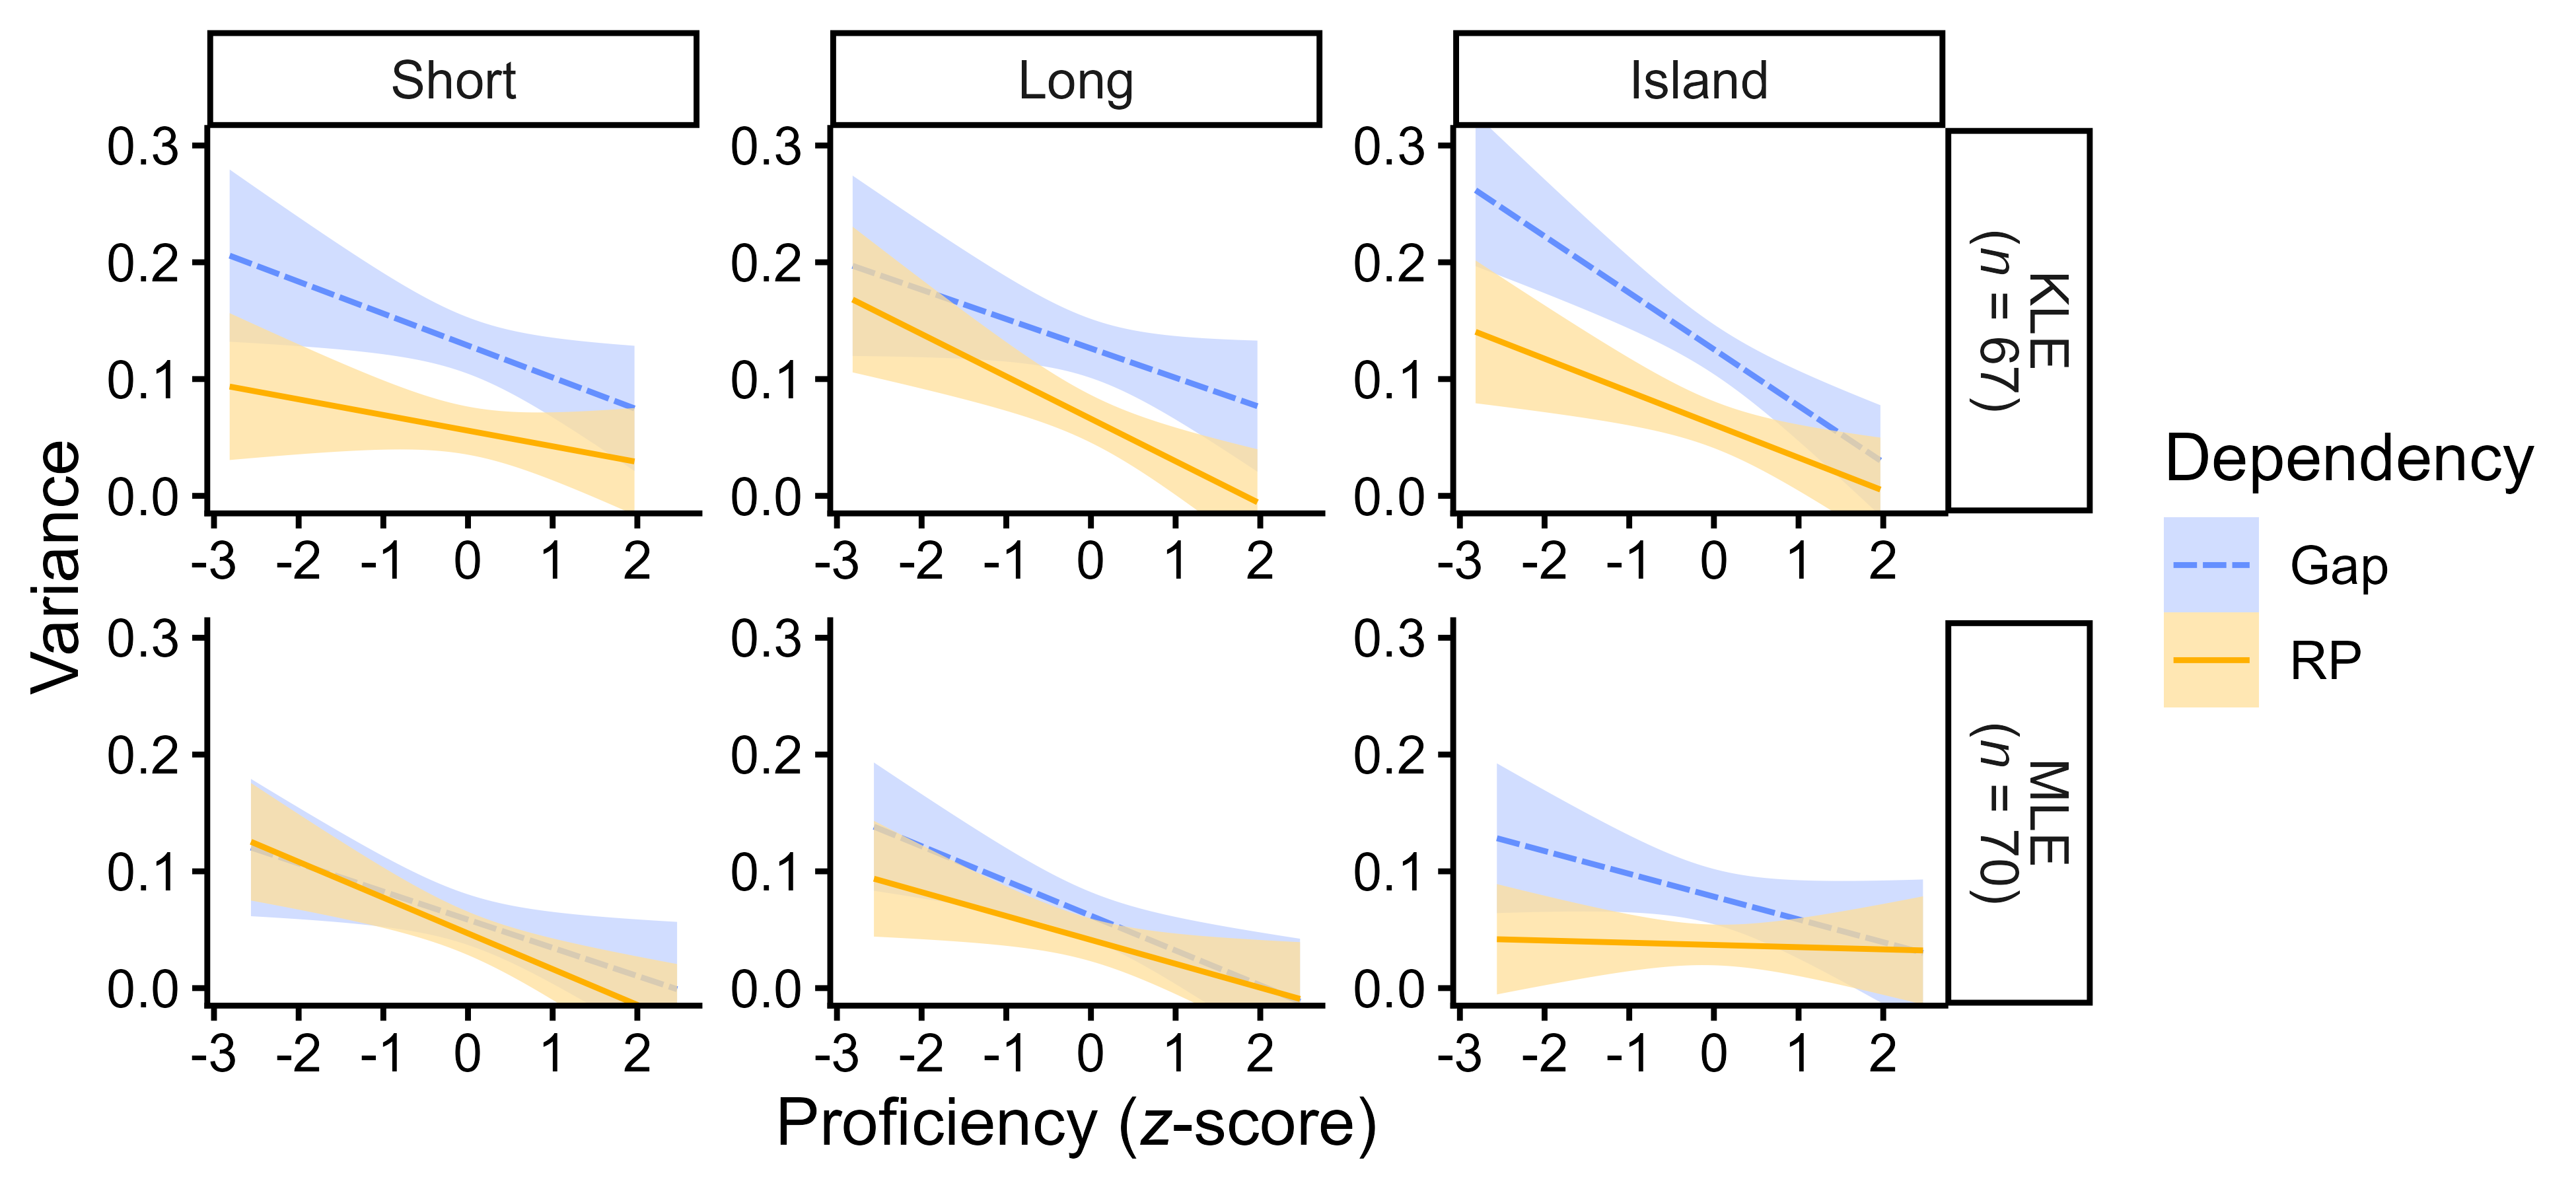
\includegraphics{../analysis/plots/orc_spr_var_proficiency.png}
\vspace{-12pt}
\end{figure}

\begin{figure}
\caption{L2 proficiency effects on variance scores in the SRC self-paced reading task} \label{fig:src-spr-var-proficiency}
\raggedright\setstretch{1}
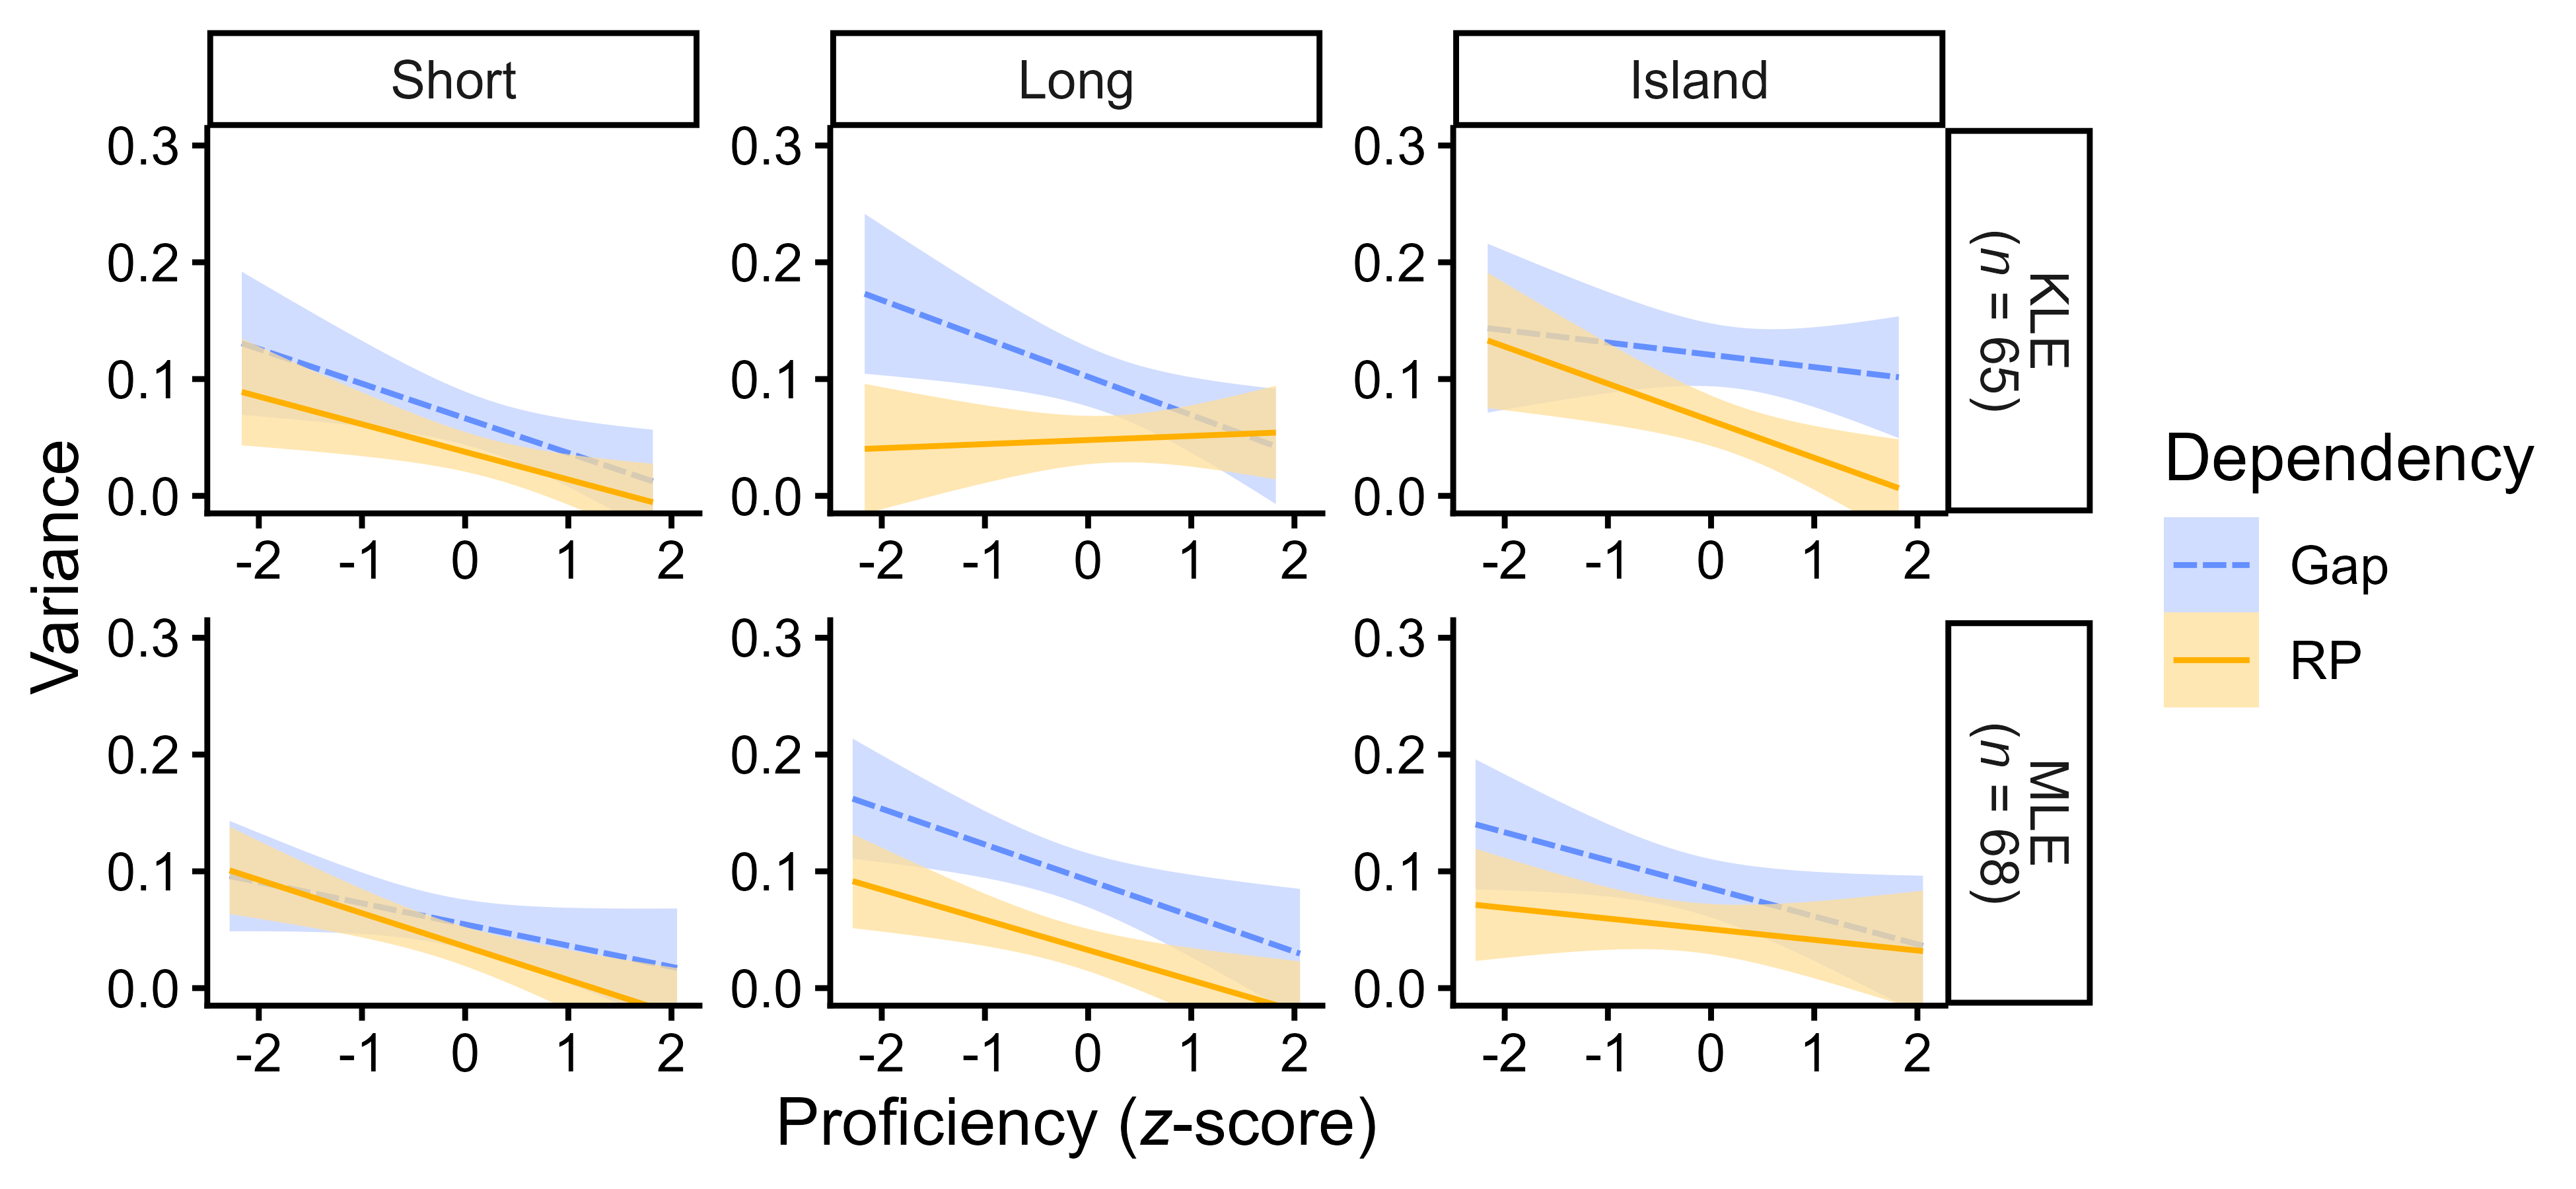
\includegraphics{../analysis/plots/src_spr_var_proficiency.png}
\vspace{-12pt}
\end{figure}

\noindent There as a strong tendency for variances to shrink as proficiency scores went up, as evidenced by the negative slopes of the regression lines in the plots. The only exception was for KLEs in the SRC Long condition, where variances appeared to increase very slightly as proficiency rose.

I further probed for proficiency effects in the SPRT variance data by refitting the linear mixed-effects models for the ORC and SRC datasets with \textsc{proficiency} added as a continuous fixed effect. The ORC model (model formula: \textsc{variance \~{} dependency * environment * group * proficiency + (1 + dependency | participant)}---see Table \ref{tblr:app-orc-spr-var-proficiency-model} in the appendices for details) yielded a significant effect for \textsc{proficiency}, with variances tending to shrink as proficiency increased ($\hat{\beta}$~=~−0.03, \textit{SE}~=~0.00, $p$~<~.001). One of the three-way \textsc{environment} × \textsc{group} × \textsc{proficiency} interactions came out as significant ($p$~=~.008), but the pairwise comparisons did not find the [RP~−~gap] contrast to be significant for any of the \textsc{environment} × \textsc{group} combinations when considered individually. 

Like the ORC model, the SRC model (model formula: \textsc{variance \~{} dependency * environment * group * proficiency + (1 + dependency + environment | participant)}---see Table \ref{tblr:app-src-spr-var-proficiency-model} in the appendices for details) found a significant effect for \textsc{proficiency}, with variances tending to shrink as proficiency increased ($\hat{\beta}$~=~−0.02, \textit{SE}~=~0.00, $p$~<~.001). Two of the three-way and four-way interactions involving \textsc{proficiency} were also in the marginally significant to significant range ($p$~<~.10). Pairwise comparisons turned up a marginally significant effect by which the RP advantage in variances shrank with rising proficiency, but only for KLEs, and only in the Long condition ($\hat{\beta}$~=~0.04, \textit{SE}~=~0.01, $p$~=~.072). 

These results indicate that processing in general becomes faster and more efficient as L2 proficiency increases. This increased efficiency in turn can decrease the facilitatory effect of resumption relative to gapping.

%========================================================%
\section{AJT variance data}\label{var-ajt}
%========================================================%

To address RQ2, I examined how variance in participants' acceptance of gaps and RPs in the AJTs patterned across the SLW hierarchy. My procedure for obtaining variance scores for the analysis was as follows. First, I transformed the raw ratings to binary acceptance scores to make them as comparable as possible to the binary accuracy scores from the analysis of the SPRT data. Ratings of 4, 5, or 6 were coded as acceptance and ratings of 1, 2, or 3 were coded as rejection. I then calculated the variance for each participant's acceptance scores in each condition. 

Figures~\ref{fig:orc-ajt-var} and \ref{fig:src-ajt-var} show the mean variance for acceptance of gaps and RPs in the ORC and SRC datasets, respectively. The variance scores were almost always at their lowest in the [Gap, Short] condition, suggesting that it was the easiest one to rate. This was to be expected because (a)~English, Korean, and Mandarin all allow gapping in short-distance RCs and (b)~the Short environment is the one the places the smallest burden on the processor. Variance scores tended to be considerably larger in all the other conditions. Unlike in the SPRT data, where variance was smaller for RPs than for gaps across all conditions, here we see that variance for RPs was generally either on par with or larger than variance for gaps, suggesting that RPs were as hard or harder to rate than gaps across all levels of the SLW hierarchy.

\begin{figure}
\caption{Mean variance for acceptance in the ORC acceptability judgment task} \label{fig:orc-ajt-var}
\raggedright\setstretch{1}
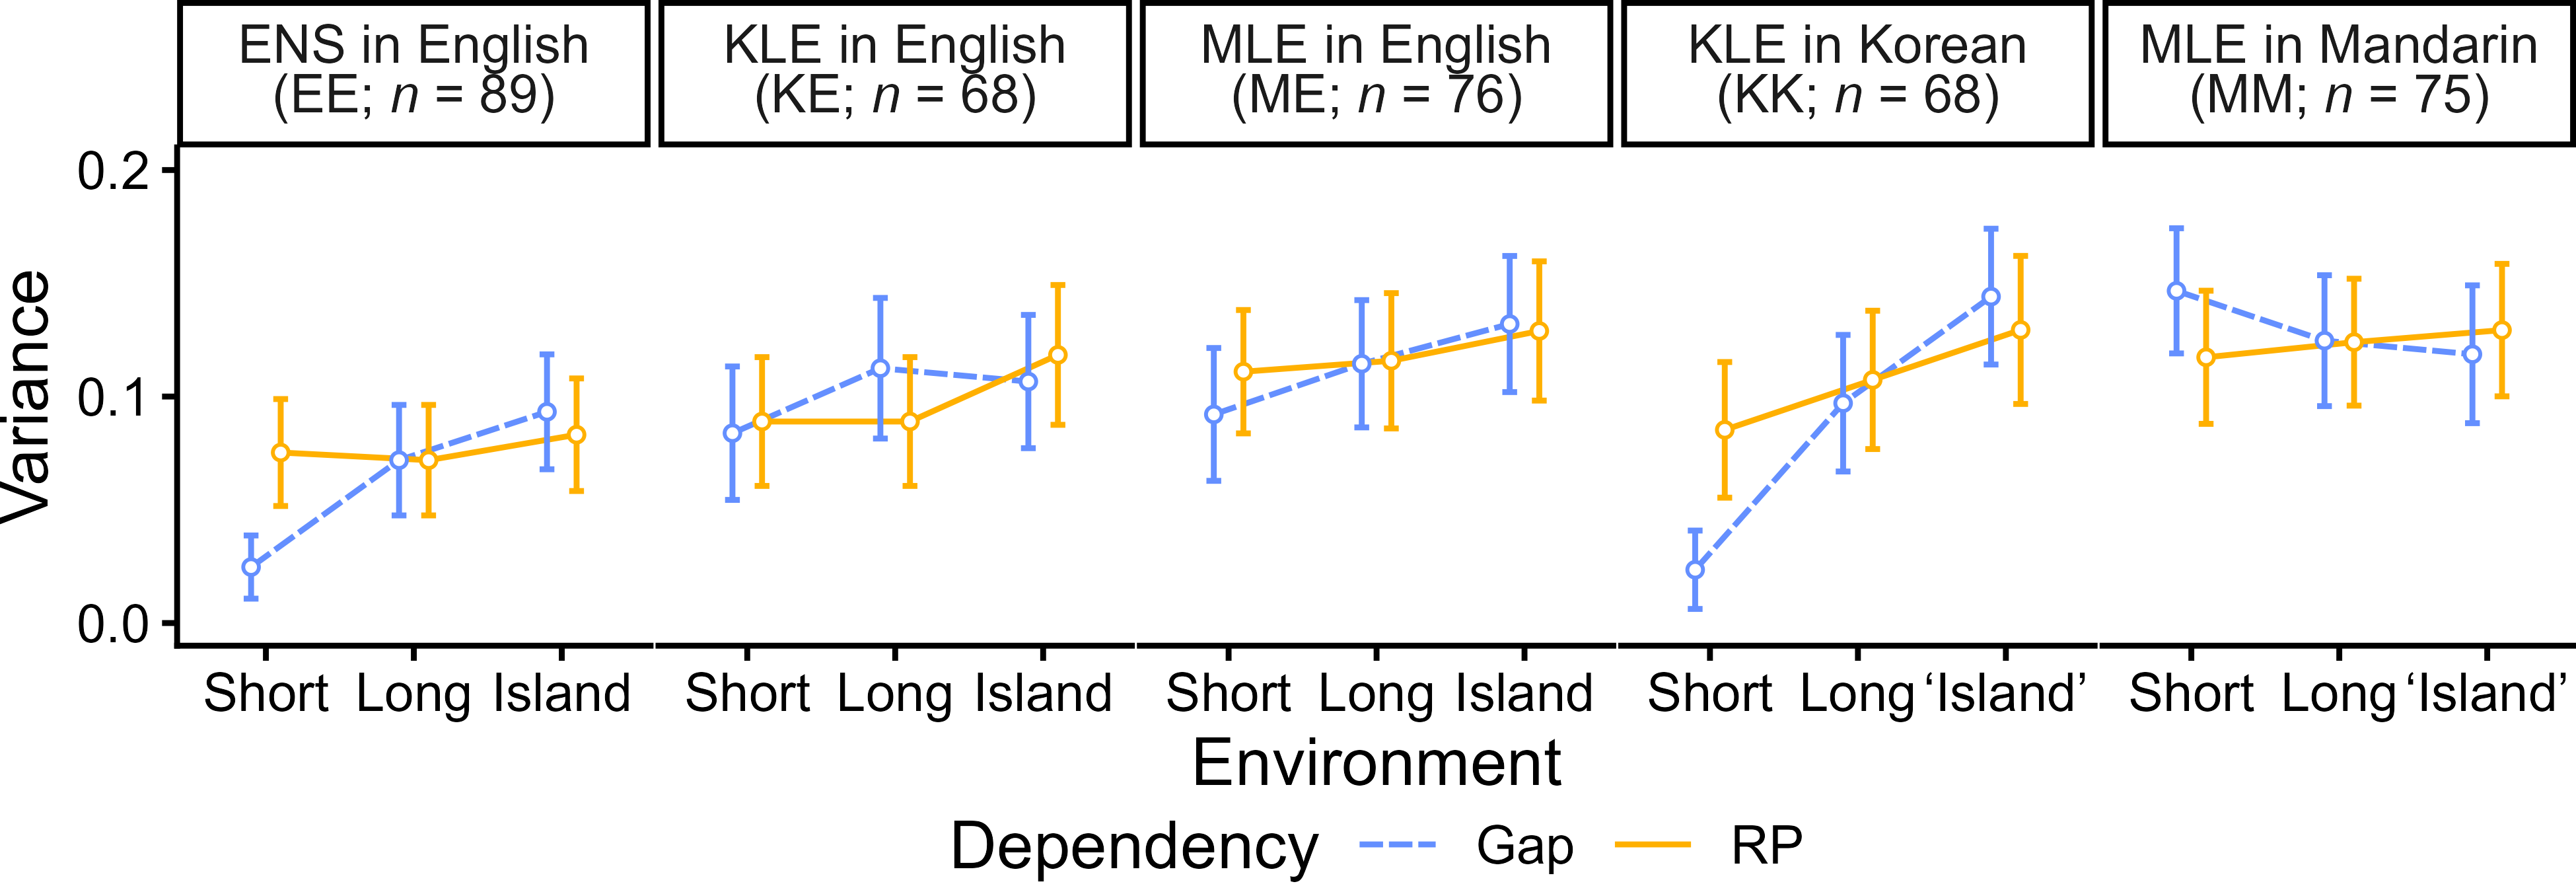
\includegraphics{../analysis/plots/orc_ajt_var.png}
\vspace{-12pt}
\end{figure}

\begin{figure}
\caption{Mean variance for acceptance in the SRC acceptability judgment task} \label{fig:src-ajt-var}
\raggedright\setstretch{1}
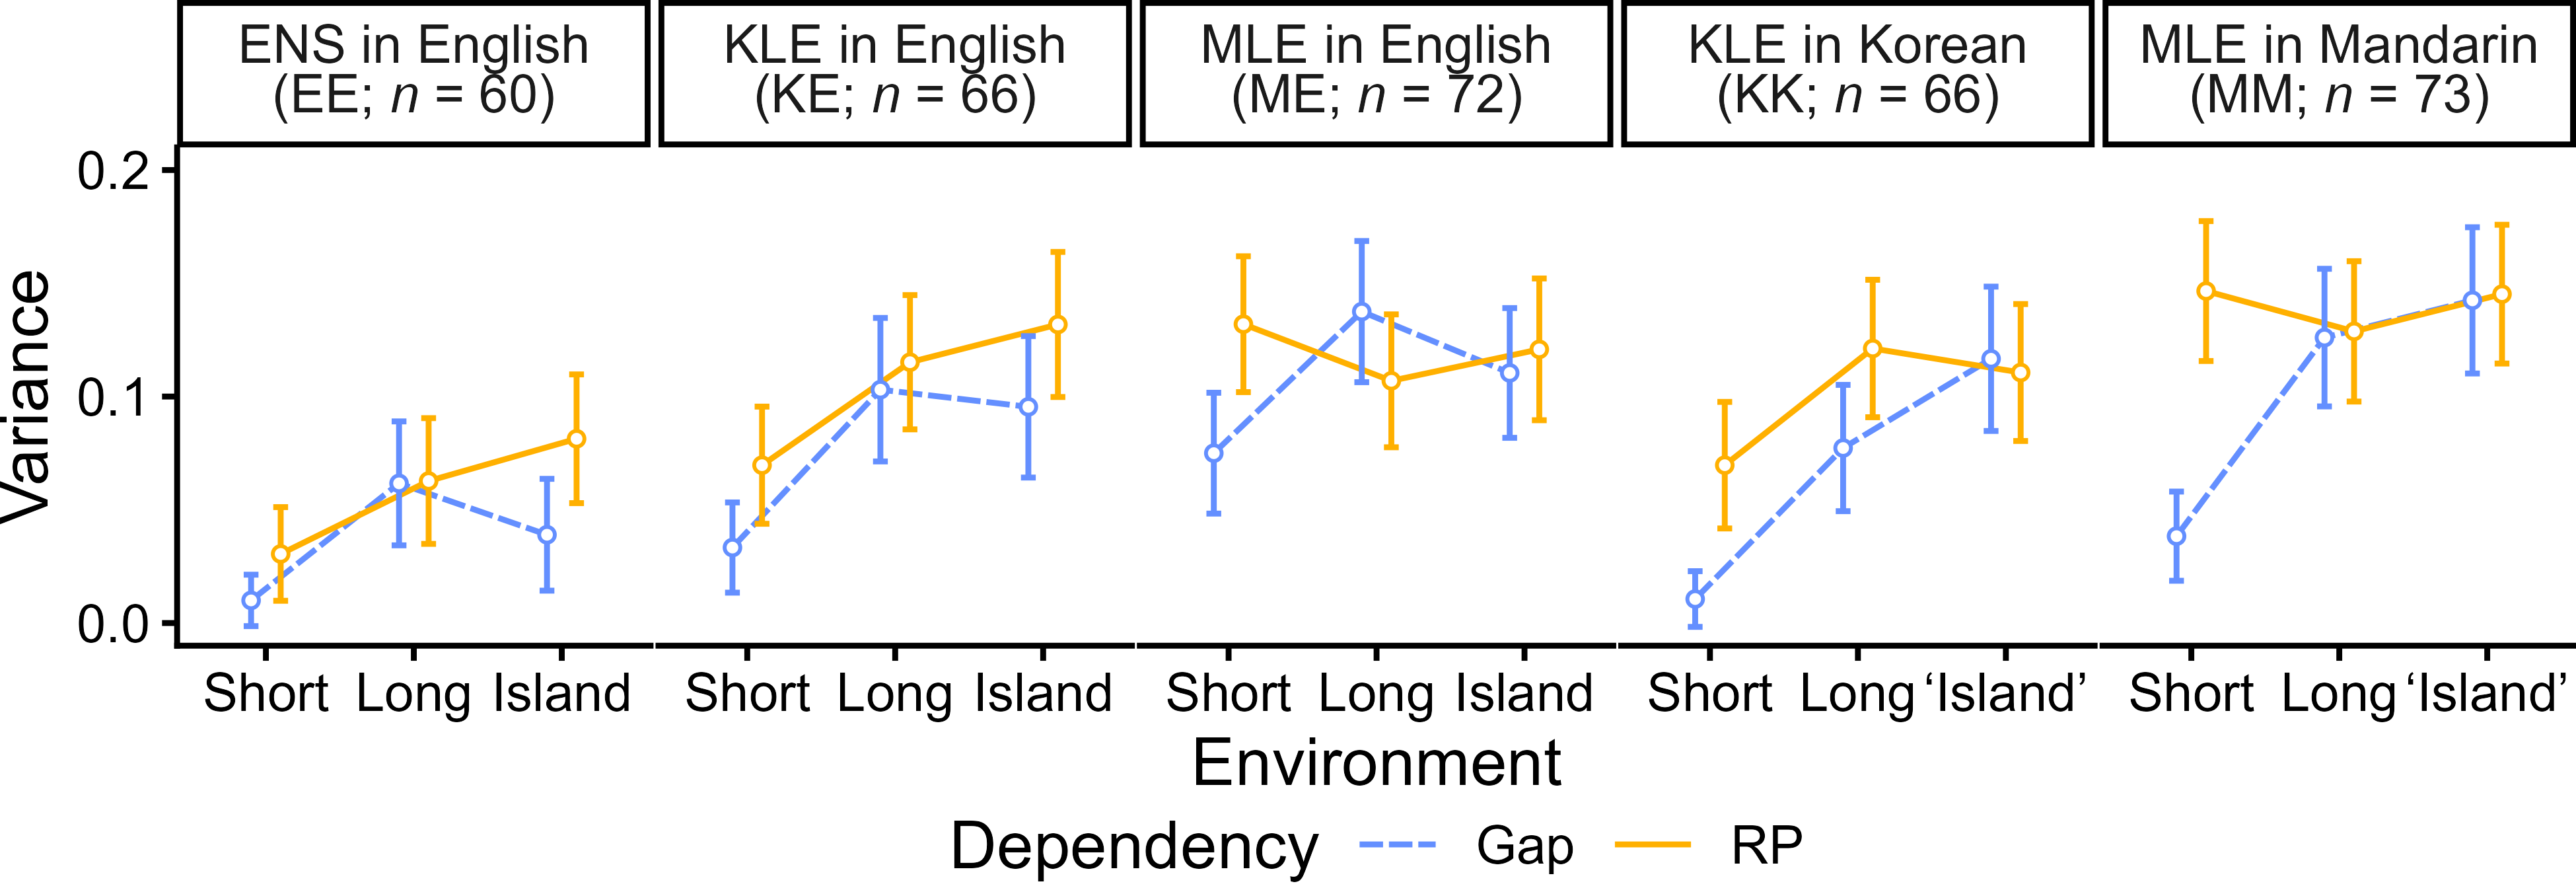
\includegraphics{../analysis/plots/src_ajt_var.png}
\vspace{-12pt}
\end{figure}

I examined the variance scores further by fitting them to separate linear mixed-effects models for the ORC and SRC datasets. The ORC model (model formula: \textsc{variance \~{} dependency * environment * pairing + (1 + dependency * environment | participant)}---see Table \ref{tblr:app-orc-ajt-var-model} in the appendices for details) did not find a significant effect for \textsc{dependency} ($p$~=~.278). However, it did turn up significant effects for \textsc{environment}, with variances being larger in the Long and Island conditions than they were in the Short condition (Long~−~Short: $\hat{\beta}$~=~0.02, \textit{SE}~=~0.01, $p$~=~.002; Island~−~Short: $\hat{\beta}$~=~0.03, \textit{SE}~=~0.01, $p$~<~.001), and for \textsc{pairing}, with variances being larger in the KE, ME, KK, and MM pairings than they were in the EE pairing (KE~−~EE: $\hat{\beta}$~=~0.03, \textit{SE}~=~0.01, $p$~=~.003; ME~−~EE: $\hat{\beta}$~=~0.05, \textit{SE}~=~0.01, $p$~<~.001; KK~−~EE: $\hat{\beta}$~=~0.03, \textit{SE}~=~0.01, $p$~=~.004; MM~−~EE: $\hat{\beta}$~=~0.06, \textit{SE}~=~0.01, $p$~<~.001). Several of the two-way and three-way interactions also reached significance ($p$~<~.05). Pairwise comparisons revealed marginally significant to significant effects whereby RP trials had more variance than gap trials, but only in the Short condition, and only in the EE and KK pairings (EE: $\hat{\beta}$~=~0.05, \textit{SE}~=~0.02, $p$~=~.057; KK: $\hat{\beta}$~=~0.06, \textit{SE}~=~0.02, $p$~=~.028). 

Unlike the ORC model, the SRC model (model formula: \textsc{variance \~{} dependency * environment * pairing + (1 + dependency * environment | participant)}---see Table \ref{tblr:app-src-ajt-var-model} in the appendices for details) found a significant effect for \textsc{dependency}, with variances being larger for RPs than for gaps ($\hat{\beta}$~=~0.03, \textit{SE}~=~0.00, $p$~<~.001). Like in the ORC model, though, there were also significant effects for \textsc{environment}, with variances being larger in the Long and Island conditions than they were in the Short condition (Long~−~Short: $\hat{\beta}$~=~0.04, \textit{SE}~=~0.01, $p$~<~.001; Island~−~Short: $\hat{\beta}$~=~0.05, \textit{SE}~=~0.01, $p$~<~.001), and for \textsc{pairing}, with variances in the KE, ME, KK, and MM pairings all being larger than those in the EE pairing (KE~−~EE: $\hat{\beta}$~=~0.04, \textit{SE}~=~0.01, $p$~<~.001; ME~−~EE: $\hat{\beta}$~=~0.07, \textit{SE}~=~0.01, $p$~<~.001; KK~−~EE: $\hat{\beta}$~=~0.04, \textit{SE}~=~0.01, $p$~<~.001; MM~−~EE: $\hat{\beta}$~=~0.07, \textit{SE}~=~0.01, $p$~<~.001). Several of the two-way and three-way interactions came out as significant, and pairwise comparisons showed that the advantage for gaps relative to RPs reached significance only in the Short condition, and only in the ME, KK, and MM pairings (ME: $\hat{\beta}$~=~0.06, \textit{SE}~=~0.02, $p$~=~.023; KK: $\hat{\beta}$~=~0.06, \textit{SE}~=~0.02, $p$~=~.024; MM: $\hat{\beta}$~=~0.11, \textit{SE}~=~0.02, $p$~<~.001).

To summarize, variance for RPs was either on par with or larger than variance for gaps across all combinations of \textsc{environment} and \textsc{group}. There were some instances in which gaps were found to have significantly less variance than RPs, but importantly RPs were never found to have significantly less variance than gaps. The fact that the RP-over-gap advantage observed in the SPRT variance data was either nullified or reversed in each environment in the AJT variance data indicates that participants experienced difficulty rating RPs that went above and beyond what can be straightforwardly explained in terms of parsing difficulty. 

%========================================================%
\section{L2 proficiency effects for the AJT variance data}\label{var-ajt-proficiency}
%========================================================%

Lastly, let us investigate the effect that L2 English proficiency had on the AJT variance data. Figures~\ref{fig:orc-ajt-var-proficiency} and \ref{fig:src-ajt-var-proficiency} show the relationship between L2ers' AJT variance scores and their scaled English proficiency scores in the ORC and SRC datasets, respectively.

\begin{figure}
\caption{L2 proficiency effects on variance scores in the ORC acceptability judgment task} \label{fig:orc-ajt-var-proficiency}
\raggedright\setstretch{1}
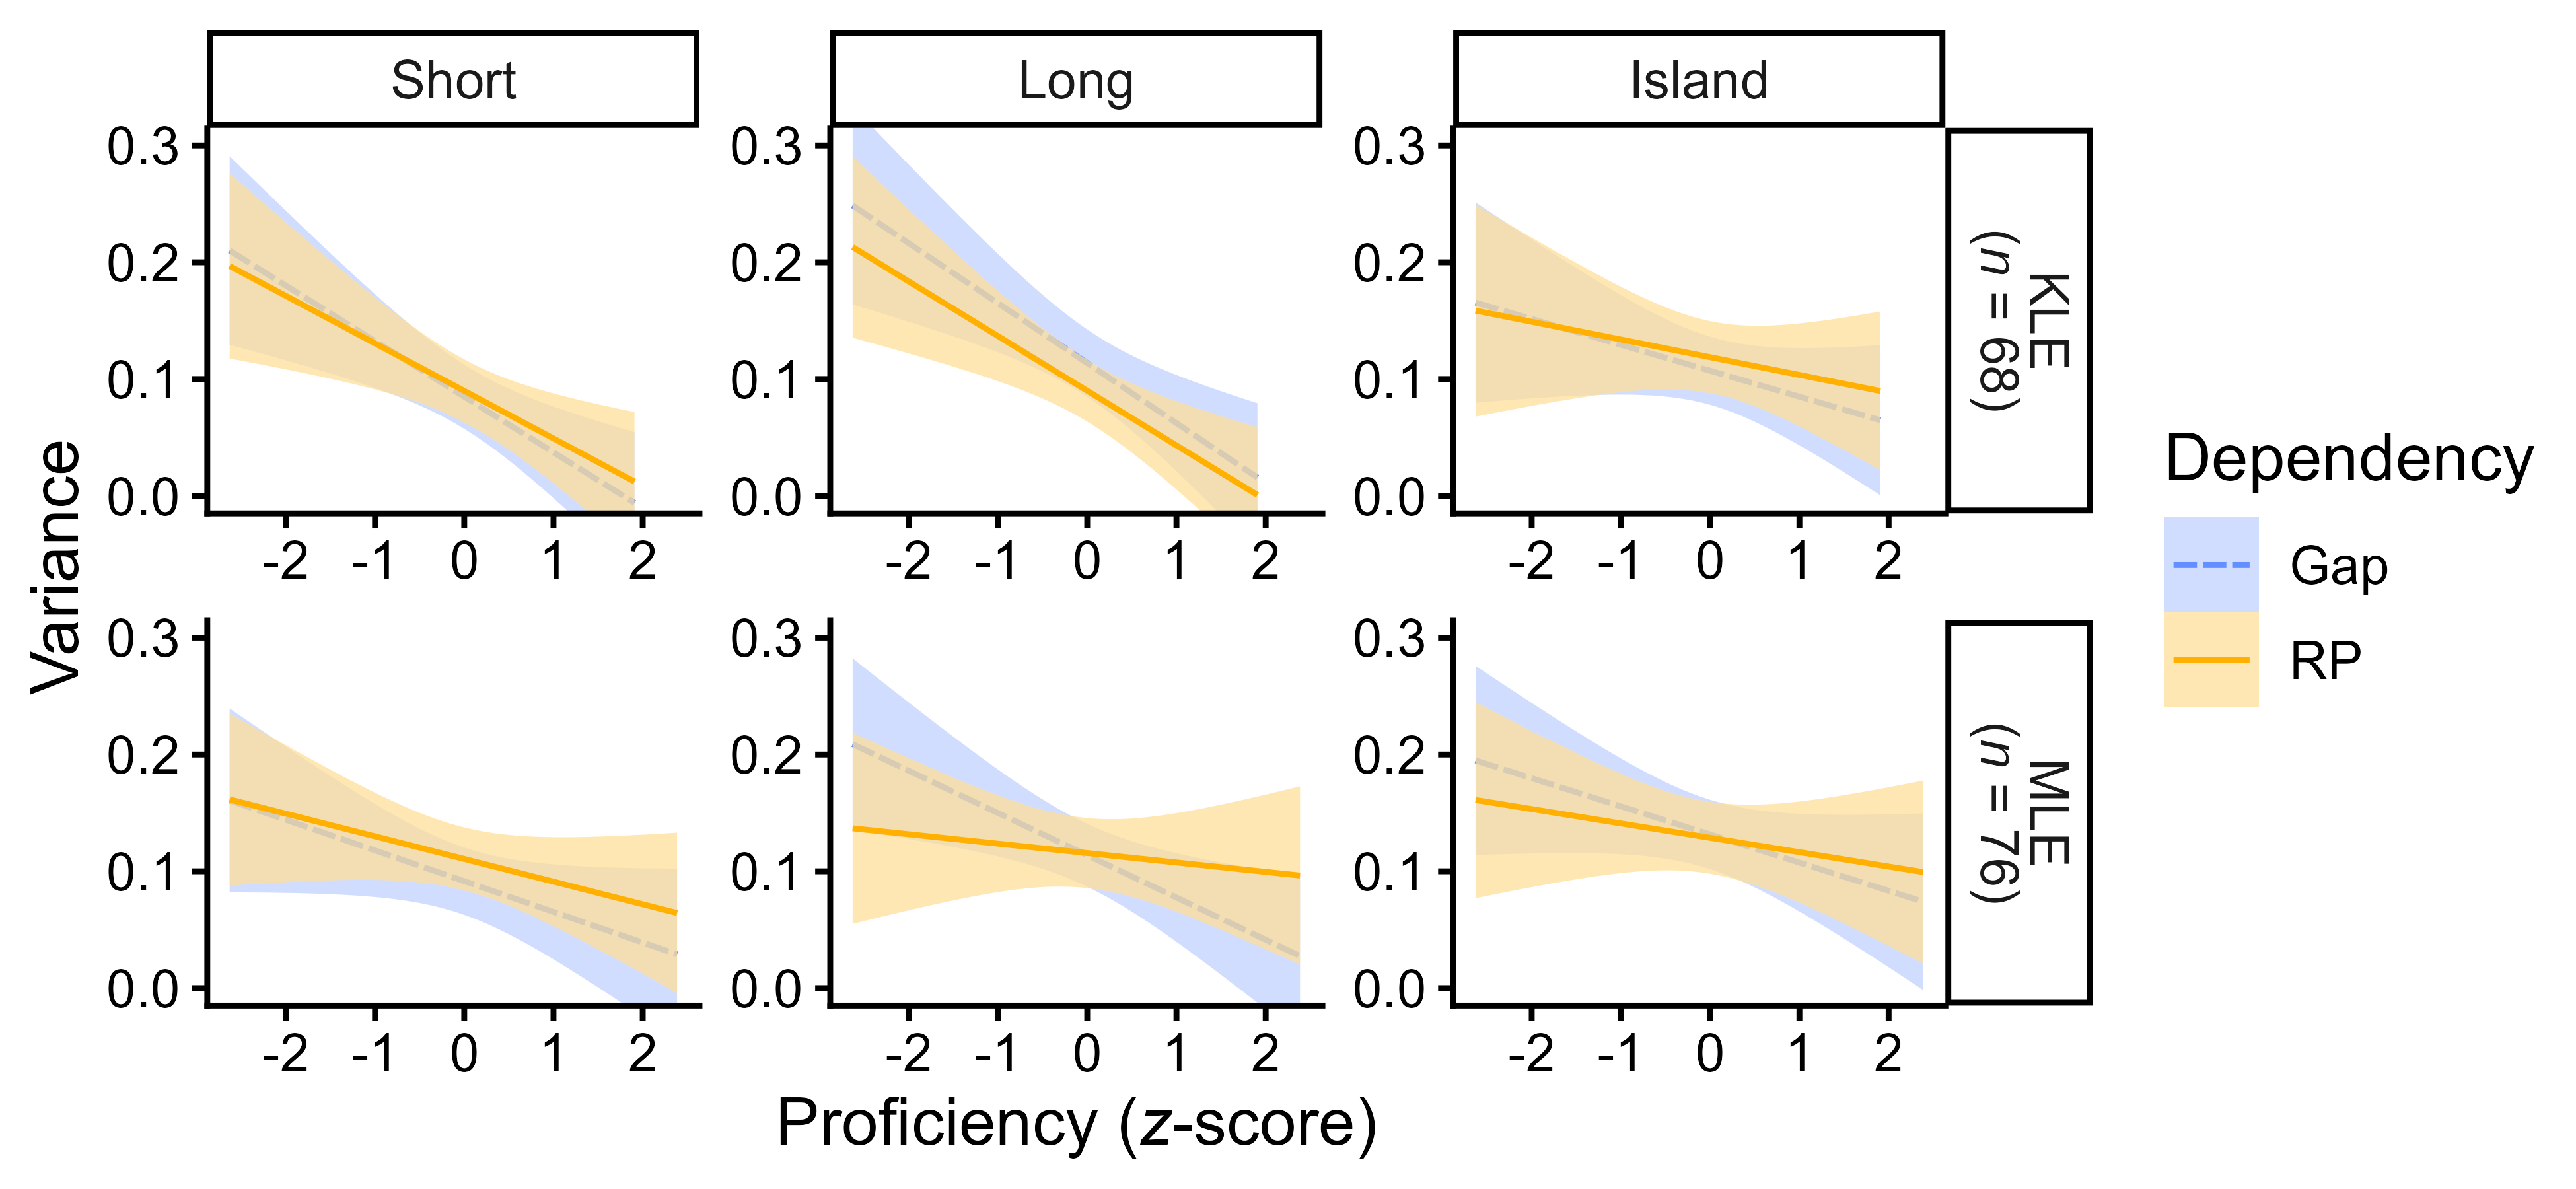
\includegraphics{../analysis/plots/orc_ajt_var_proficiency.png}
\vspace{-12pt}
\end{figure}

\begin{figure}
\caption{L2 proficiency effects on variance scores in the SRC acceptability judgment task} \label{fig:src-ajt-var-proficiency}
\raggedright\setstretch{1}
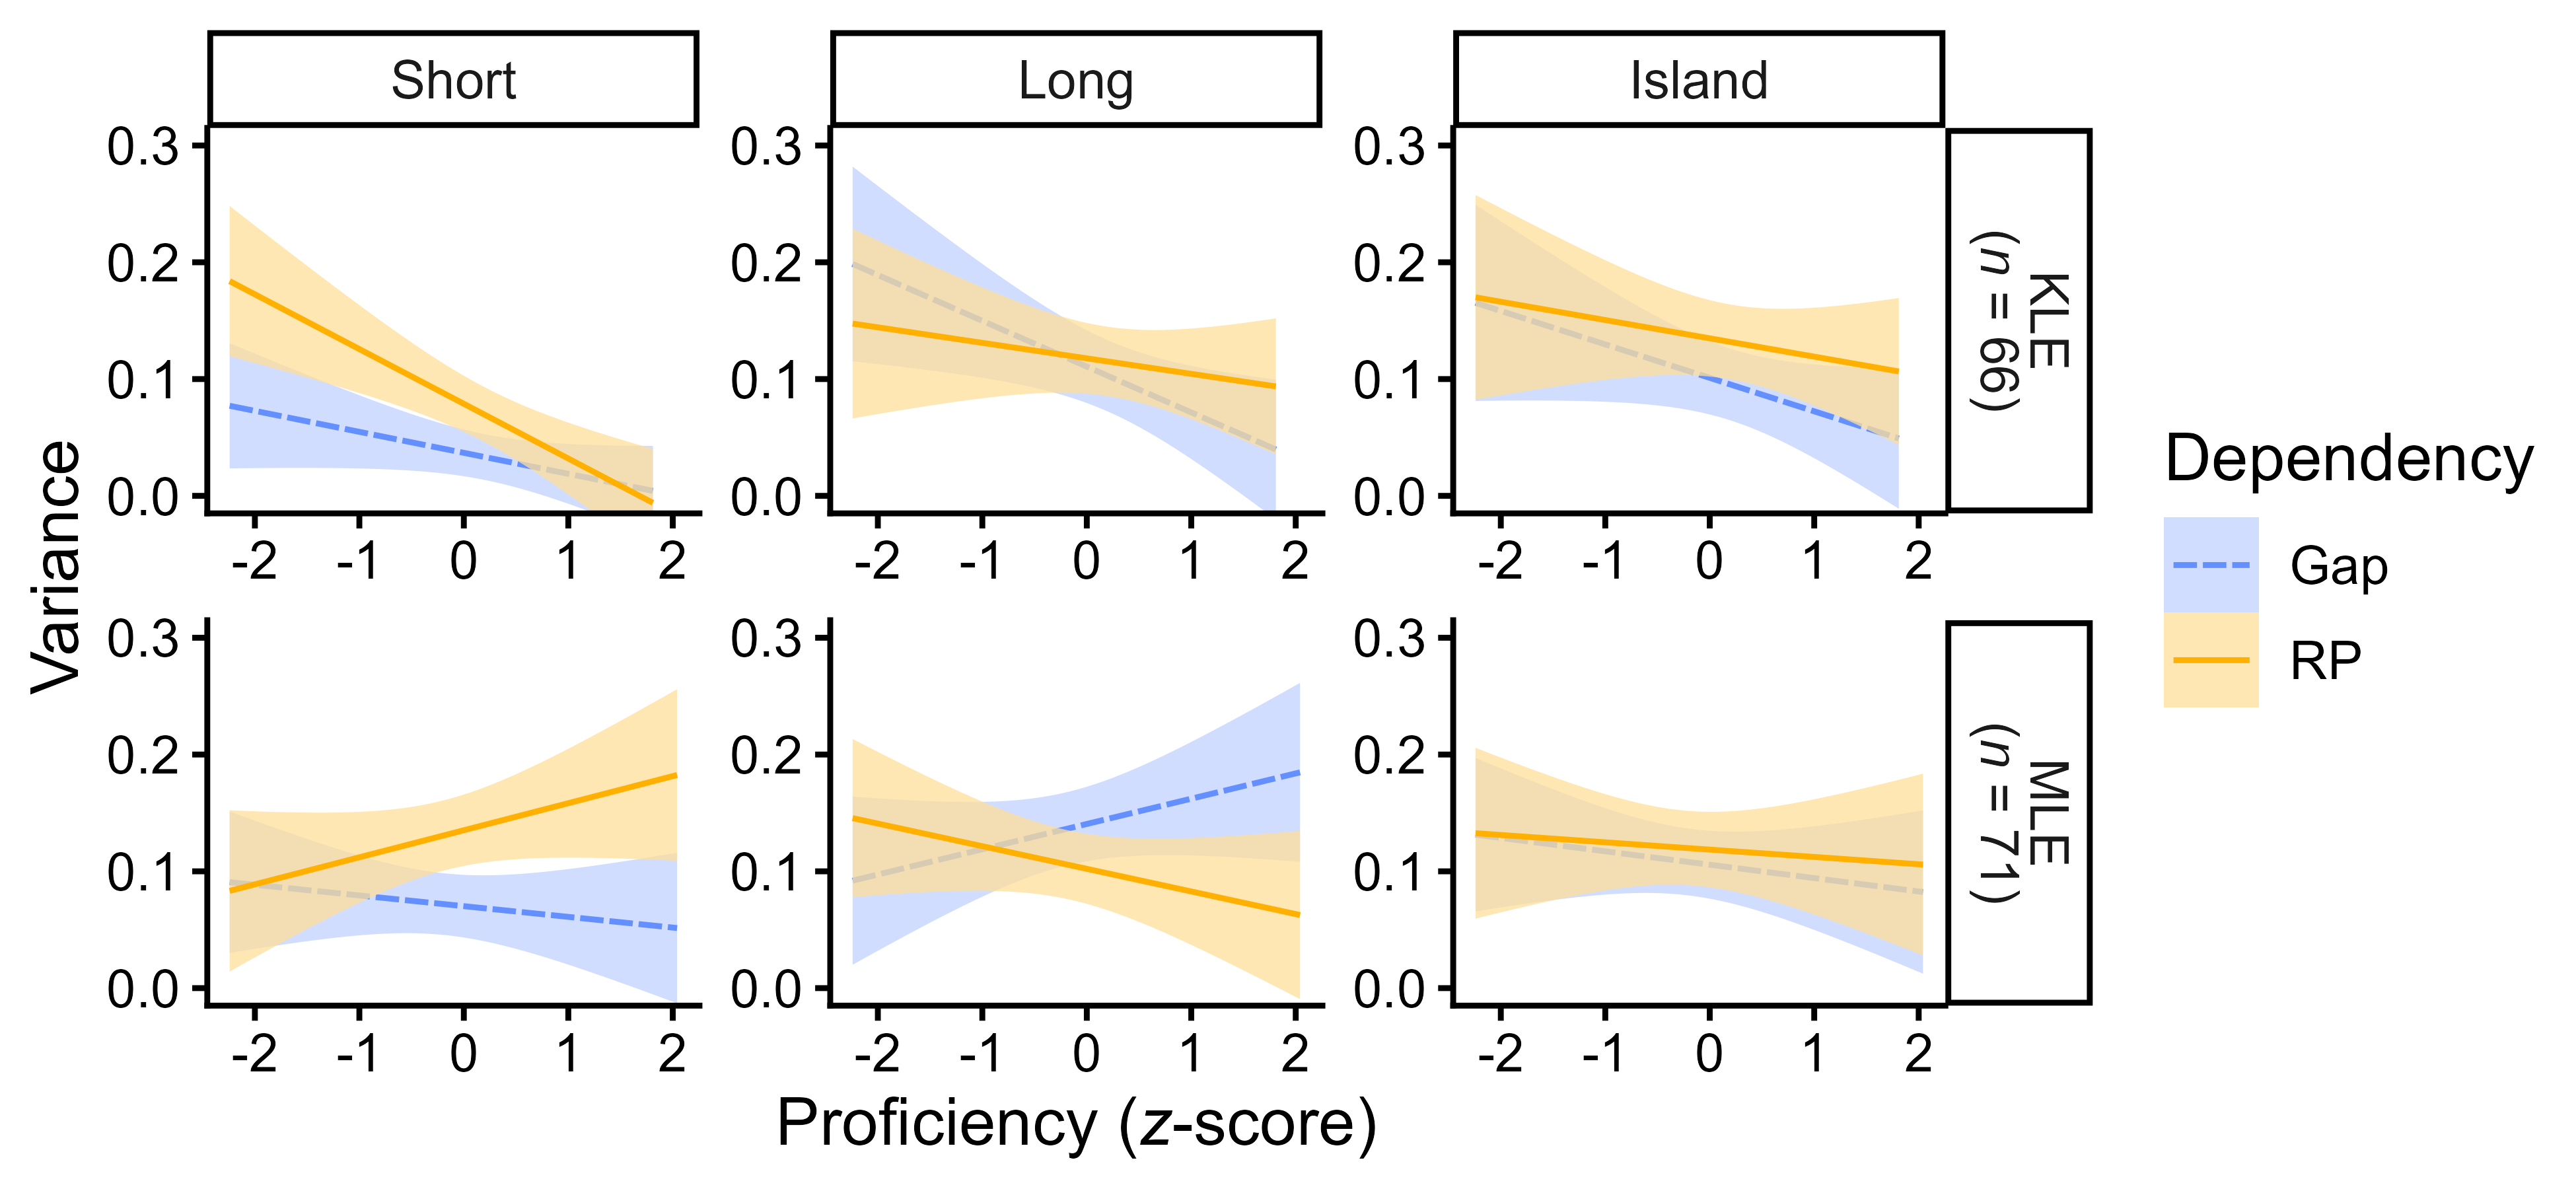
\includegraphics{../analysis/plots/src_ajt_var_proficiency.png}
\vspace{-12pt}
\end{figure}

Like in the SPRT variance data, there was a strong tendency for variance to decrease as proficiency scores became higher. The only exceptions were for MLEs in the SRC [RP, Short] and [Gap, Long] conditions, where the opposite trend was observed. In all other cases, variance for both gaps and RPs decreased with rising proficiency, suggesting that higher-proficiency participants found the sentences easier to rate than lower-proficiency ones did.

I continued to probe for proficiency effects in the AJT variance data by refitting the linear mixed-effects models for the ORC and SRC datasets with \textsc{proficiency} added as a continuous fixed effect. The ORC model (model formula: \textsc{variance \~{} dependency * environment * pairing * proficiency + (1 + dependency + environment | participant)}---see Table \ref{tblr:app-orc-ajt-var-proficiency-model} in the appendices for details) yielded a significant effect for \textsc{proficiency}, with variances tending to shrink as proficiency increased ($\hat{\beta}$~=~−0.03, \textit{SE}~=~0.01, $p$~<~.001). None of the interactions involving \textsc{proficiency} approached significance (all $p$s~>~.10), though, suggesting that the proficiency trend did not vary in a statistically meaningful way across levels of \textsc{dependency}, \textsc{environment}, and \textsc{pairing}.

Like the ORC model, the SRC model (model formula: \textsc{variance \~{} dependency * environment * pairing * proficiency + (1 + dependency + environment | participant)}---see Table \ref{tblr:app-src-ajt-var-proficiency-model} in the appendices for details) found a significant effect for \textsc{proficiency} ($\hat{\beta}$~=~−0.01, \textit{SE}~=~0.01, $p$~=~.015). Several of the two-way and four-way interactions involving \textsc{proficiency} also came out as significant ($p$~<~.05). However, post-hoc tests did not find the effect of \textsc{proficiency} on the size of the [RP~−~gap] contrast in variance scores to approach significance for any combination of \textsc{environment} and \textsc{pairing} (all $p$s~>~.10).

The fact that variances overwhelmingly tended to shrink as proficiency scores went up shows that higher-proficiency L2ers are more consistent in their ratings than their lower-proficiency peers. On the assumption that larger amounts of variance reflect greater degrees of difficulty, we can also conclude that higher-proficiency participants found the sentences easier to rate than lower-proficiency ones did. These results are consistent with perceptions of well-formedness becoming more sharply defined as proficiency increases.

%========================================================%
\section{Summing up}\label{var-conclusion}
%========================================================%

There are two main findings that emerged from the data analyses in this chapter. First, I showed that there were clear signs of processing facilitation for resumption in the SPRT variance data but not in the AJT variance data. Whereas variances were often smaller for RPs than for gaps in the SPRT data, variances for RPs were either on par with or larger than variances for gaps in the AJT data. I take these results as evidence that participants had trouble assigning ratings to resumptive RCs that went above and beyond what can be attributed to parsing difficulty alone. Instead, there appears to be another source of difficulty, which we might call a `low-entrenchment' cost, that comes into play when one is asked to rate sentence types that are parsable yet have rarely or never been encountered in the input. 

Second, I showed that higher L2 English proficiency scores were associated with lower amounts of variance in the SPRT data and the AJT data alike. The same proficiency effect was observed in all conditions and across all participant groups, with only very rare exceptions across all combinations of \textsc{dependency}, \textsc{environment}, \textsc{group}, and \textsc{study}. These results indicate, for starters, that processing becomes more efficient as proficiency increases. In the case of the AJT data, the results additionally suggest that perceptions of well-formedness come into sharper focus as an L2er's proficiency level rises. 

Both of these findings are compatible with the entrenchment approach to restructuring outlined in Section~\ref{acq-entrenchment}, according to which perceptions of well-formedness crystallize over time in response to increased exposure to target language input. It would be hard, I believe, to reconcile these findings with the flip-of-the-switch approach to restructuring, according to which well-formedness perceptions should be discrete at all stages of development and therefore there should be no difficulty associated with rating sentences beyond what can be explained in terms of parsing problems. Although it is true that other factors, such as pragmatic appropriateness, also play a role in acceptability judgments, such influences were controlled for in the current experiments by using essentially identical stimuli across the SPRTs and the AJTs.

This marks the end of the experimental portion of the dissertation. In the next and last chapter, I discuss the findings from the various experiments and conclude the dissertation.